\documentclass[a4paper,10pt]{report}
\usepackage[utf8]{inputenc}
\usepackage[francais]{babel}
\usepackage[top=1.5cm, bottom=1.5cm, left=1cm, right=1cm]{geometry}
\usepackage{graphicx}

% Title Page
\title{OMGL4 - Etape 3 : expression des besoins, analyse et conception des autres cas d'utilisation}
\author{MAILLET Arnaud (chef de projet), VARGAS Christophe, ARDAUD Guillaume}


\begin{document}
\maketitle
\newpage
\null
\newpage
\tableofcontents
\newpage
\null
\newpage

\centering

\chapter*{Nouveau numéro périodique}
\addcontentsline{toc}{chapter}{Nouveau numéro périodique}
\section*{Diagramme de séquence haut niveau}
\addcontentsline{toc}{section}{Diagramme de séquence haut niveau}

Auteur : Arnaud MAILLET
Relecteur : xx

\bigskip

\section*{Scenario principal}
\addcontentsline{toc}{section}{Scenario principal}
\begin{flushleft}
- La documentaliste demande l'enregistrement pour une nouvelle parution d'un périodique donné.\\
- Le système demande le numéro ISSN du périodique.\\
- La documentaliste saisit le numéro ISSN du périodique.\\
- Le système recherche le périodique dans le système informatique et affiches ses informations propres (nom périodique).\\
- Le système demande le numéro de parution de la nouvelle parution.\\
- La documentaliste saisit le numéro de parution de la nouvelle parution\\
- Le système créé la nouvelle parution et lie la nouvelle parution à son periodique.\\
- Le système demande les informations propres des articles de la parution (titre, page, auteurs, mots clés).\\
- La documentaliste saisit les informations propres des articles de la parution.\\
- Le système crée les articles et lie les articles à la parution du periodique.
- Le système confirme l'enregistrement de la nouvelle parution.\\
\end{flushleft}

\bigskip

\section*{Diagramme de séquence haut niveau}
\addcontentsline{toc}{section}{Diagramme de séquence haut niveau}
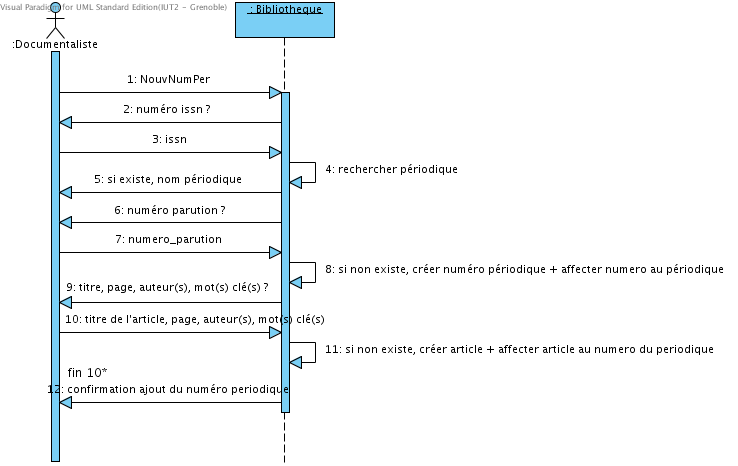
\includegraphics[height=115mm]{NouvNumPerHautNiveau.png}

\newpage

\section*{Unité de présentation}
\addcontentsline{toc}{section}{Unité de présentation}
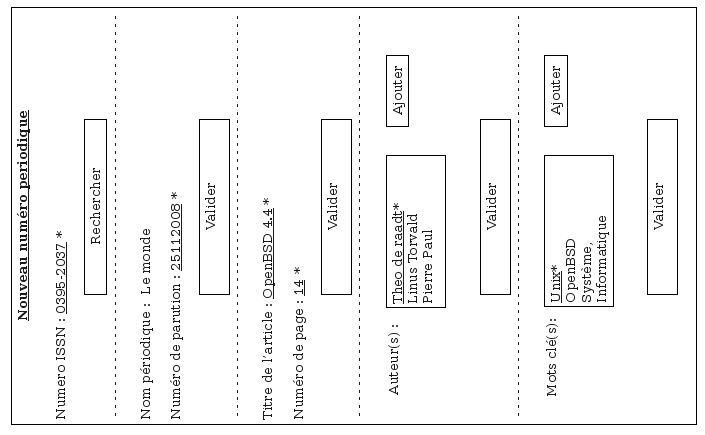
\includegraphics[height=70mm]{UpNouvNumPer.png}

\section*{Diagramme de séquence détaillé MVC}
\addcontentsline{toc}{section}{Diagramme de séquence détaillé MVC}
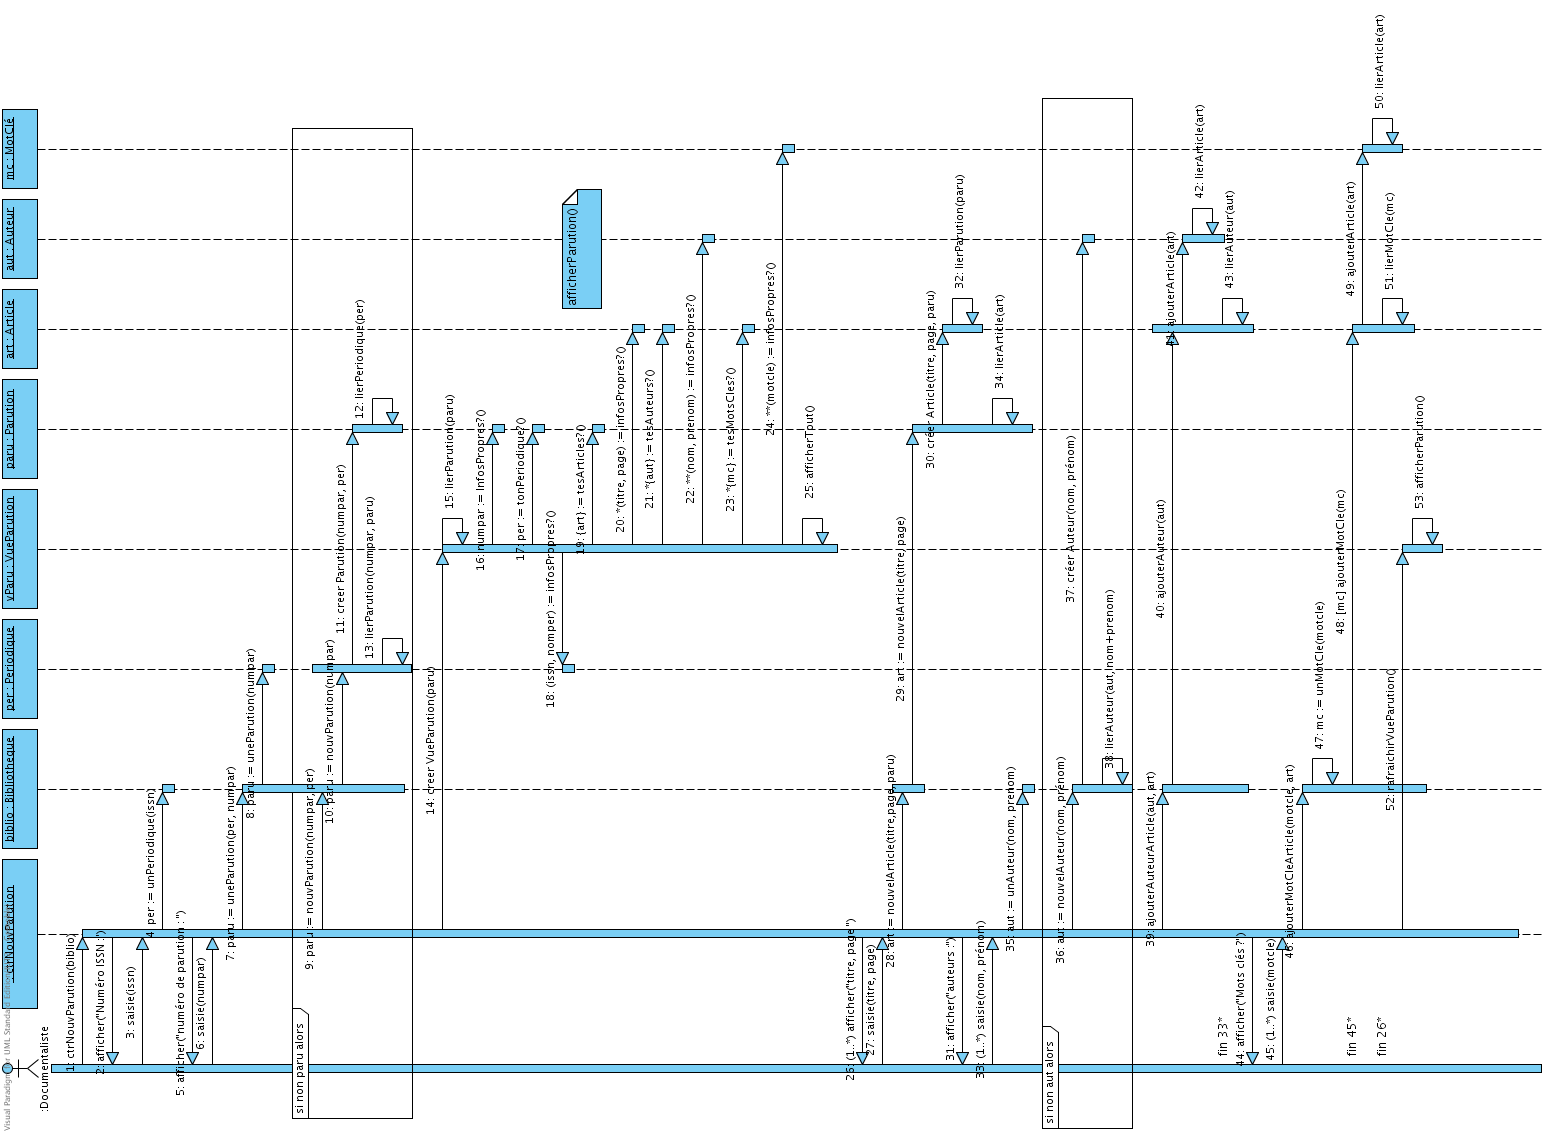
\includegraphics[height=170mm]{NouvNumPerMVC.png}


\end{document}
